\documentclass{beamer}
\definecolor{links}{HTML}{2A1B81}
\hypersetup{colorlinks,linkcolor=,urlcolor=links}
\usepackage{tikz}
\usetikzlibrary{decorations.pathreplacing}
\usetikzlibrary{decorations.pathmorphing}
\usetikzlibrary{arrows}
\usetikzlibrary{decorations.markings}
\usetikzlibrary{decorations.pathreplacing}
\usetikzlibrary{backgrounds}
\usetikzlibrary{calc}
\usetikzlibrary{intersections}
\usetikzlibrary{decorations}
\usetikzlibrary{shapes, positioning} 
\usetikzlibrary{shadows}
\usepackage{relsize}
\tikzset{fontscale/.style = {font=\relsize{#1}}
}
\tikzstyle{line}=[draw,thick,-latex]
\setbeamerfont{block title}{size=\large}
\setbeamerfont{frametitle}{size=\Huge}
\setbeamertemplate{frametitle}[default][center]

%
% Choose how your presentation looks.
%
% For more themes, color themes and font themes, see:
% http://deic.uab.es/~iblanes/beamer_gallery/index_by_theme.html
%
\mode<presentation>
{
  \usetheme{default}      % or try Darmstadt, Madrid, Warsaw, ...
  \usecolortheme{default} % or try albatross, beaver, crane, ...
  \usefonttheme{default}  % or try serif, structurebold, ...
  \setbeamertemplate{navigation symbols}{}
  \setbeamertemplate{caption}[numbered]
} 

\usepackage[english]{babel}
\usepackage[utf8x]{inputenc}

\title[]{Timepix3 in the AEgIS experiment}
\author{Helga Holmestad}
\institute{University of Oslo}
\date{19/9-2018}

\begin{document}

\begin{frame}
  \titlepage
\end{frame}

% Uncomment these lines for an automatically generated outline.
%\begin{frame}{Outline}
%  \tableofcontents
%\end{frame}

\section{Introduction}

\begin{frame}{\centering AEgIS experiment}
  \begin{columns}
    \begin{column}{0.5\textwidth}
      \begin{itemize}
      \item{Measure the gravitational acceleration of antimatter}
      \item{Test if the  weak equivalence principle holds also for antimatter}
      \end{itemize}
     \end{column}
    \begin{column}{0.5\textwidth}
      \begin{figure}
        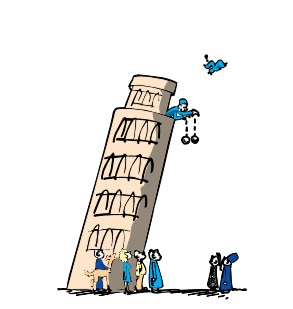
\includegraphics[width=\textwidth]{fig/gali3.jpg}
        \end{figure}
    \end{column}
  \end{columns}
  

%\vskip 1cm

%\begin{block}{Examples}

  
%\end{block}

\end{frame}


\begin{frame}{\centering A classical moiré deflectometer}
  %% \begin{columns}
  %%   \begin{column}{0.4\textwidth}
  %%     \begin{itemize}
  %%     \item Measure the gravitational accelration of antimatter
  %%     \item Test weak equivalence principle
  %%     \end{itemize}
  %%    \end{column}
  %%   \begin{column}{0.8\textwidth}
  \begin{tikzpicture}
    \node at (0,0) {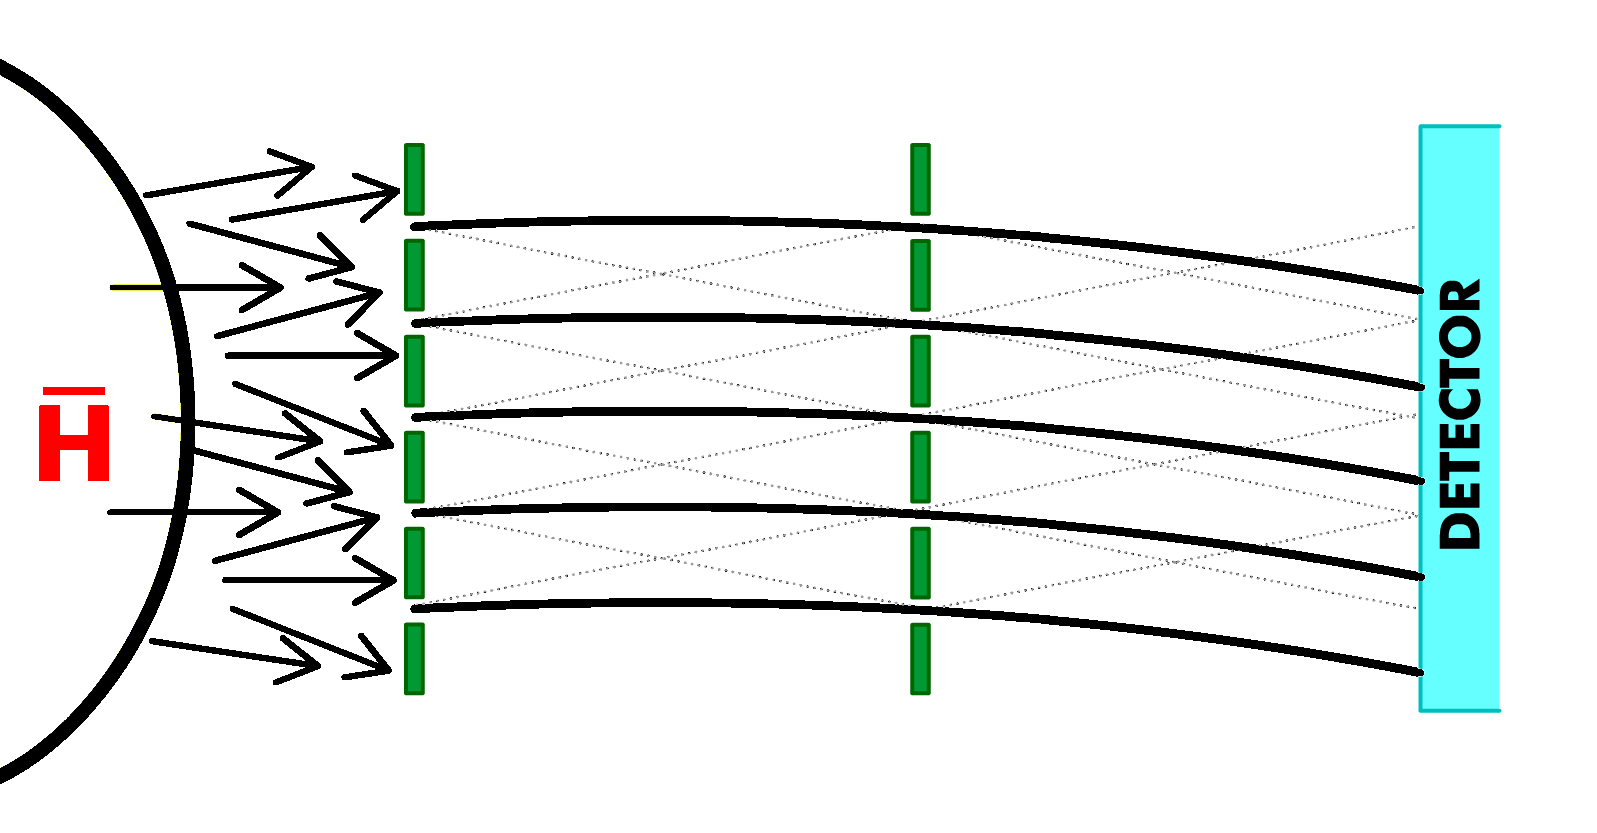
\includegraphics[width=\textwidth]{fig/moire.png}};
    \visible <2> {\node[star, star points=5, minimum width=0.1cm,inner sep=1.8pt,anchor=outer point 3,star point ratio=5.25, fill=yellow, draw] at (4,0.5) {};
      \node[star, star points=5, minimum width=0.1cm,inner sep=1.8pt,anchor=outer point 3,star point ratio=5.25, fill=yellow, draw] at (4,-0.2) {};
      \node[star, star points=5, minimum width=0.1cm,inner sep=1.8pt,anchor=outer point 3,star point ratio=5.25, fill=yellow, draw] at (4,-0.85) {};
     \node[star, star points=5, minimum width=0.1cm,inner sep=1.8pt,anchor=outer point 3,star point ratio=5.25, fill=yellow, draw] at (4,-1.5) {};
     \node[star, star points=5, minimum width=0.1cm,inner sep=1.8pt,anchor=outer point 3,star point ratio=5.25, fill=yellow, draw] at (4,-2.15) {};
      }
    %\node[star,fill=red,minimum width=0.2cm] at (0,0) {};
    %\visible <2> {\node at (6,0) {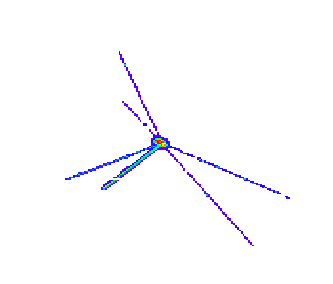
\includegraphics[width=0.4\textwidth]{fig/antiprotonExTest.png}};}
    %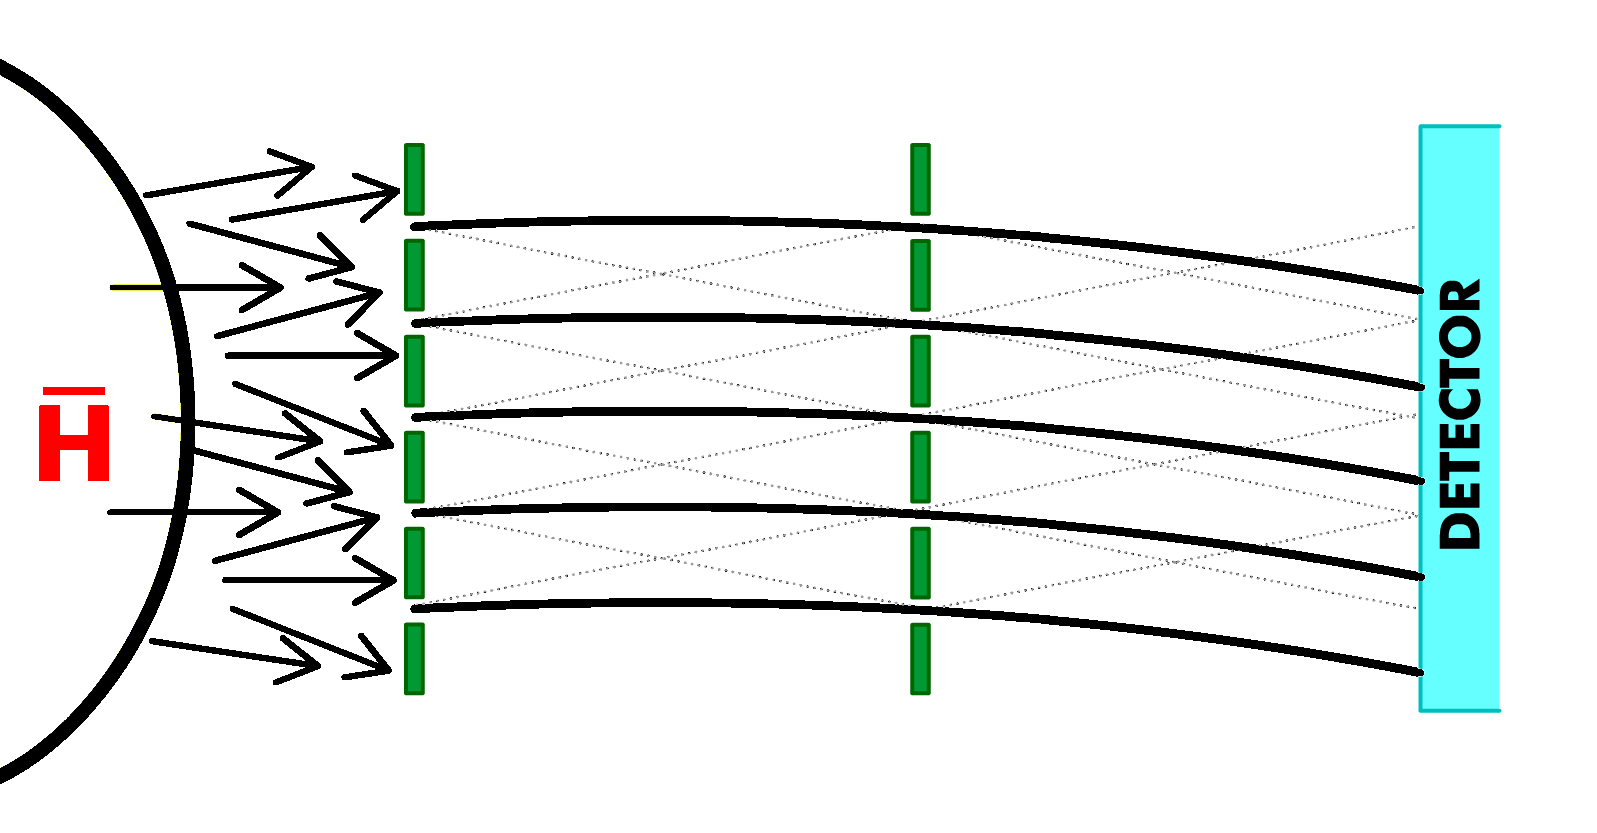
\includegraphics[width=0.8\textwidth]{fig/moire.jpg}
  \end{tikzpicture}
  %%   \end{column}
  %% \end{columns}
\end{frame}

\begin{frame}{\centering Requirements for the detector}  
  %% \begin{columns}
  %%   \begin{column}{0.4\textwidth}
  \begin{itemize}
    \item{Tag antihydrogen}
      \visible<2->{
        \begin{itemize}
        \item{Fragments from annihilations outside the detector}
%        \item{Trade off between tagging efficiency and purity of sample}
        \end{itemize}
      }
  \item{Measure time of flight}
    \visible<3->{\begin{itemize}
      \item{Energy of antihydrogen beam will not be completely uniform}
      \item{Transit time through the moirè deflectometer is around 2ms}
      \end{itemize}
      }
  \item{Reconstruct the annihilation point}
    \visible<4->{\begin{itemize}
      \item{The shift of pattern is 10~$\mu$m -- 20~$\mu$m}
      \item{Around 10~$\mu$m resolution needed to achieve 1\% precision on $\bar g$}
      \end{itemize}
      }
    \end{itemize}
  %%    \end{column}
  %%   \begin{column}{0.8\textwidth}
  %\begin{figure}
  %  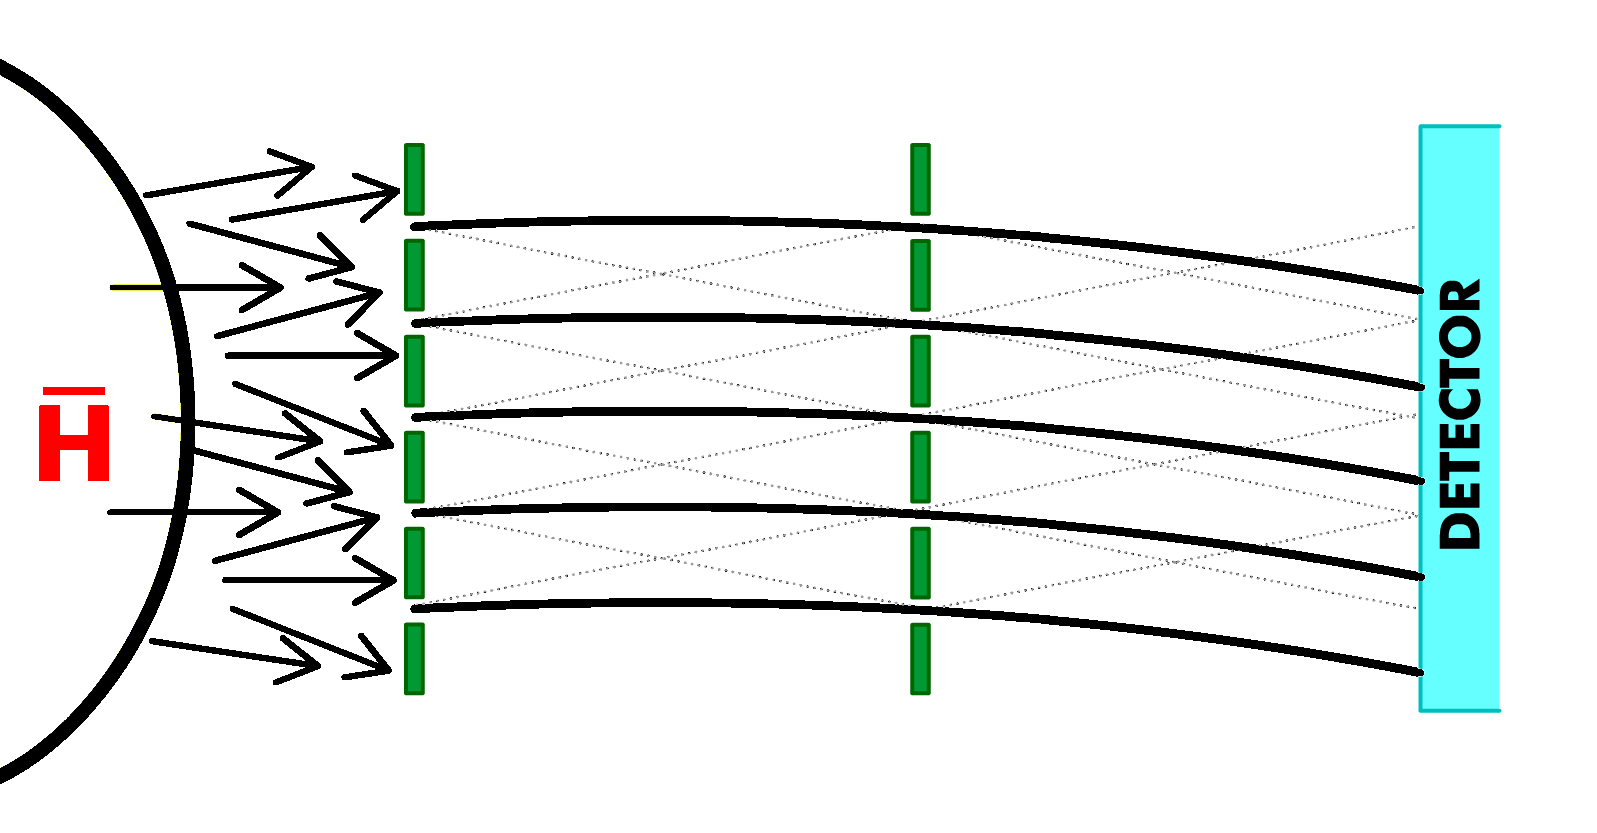
\includegraphics[width=0.8\textwidth]{fig/moire.png}
  %\end{figure}
  %%   \end{column}
  %% \end{columns}
\end{frame}


\begin{frame}{\centering GRACE beamline}
        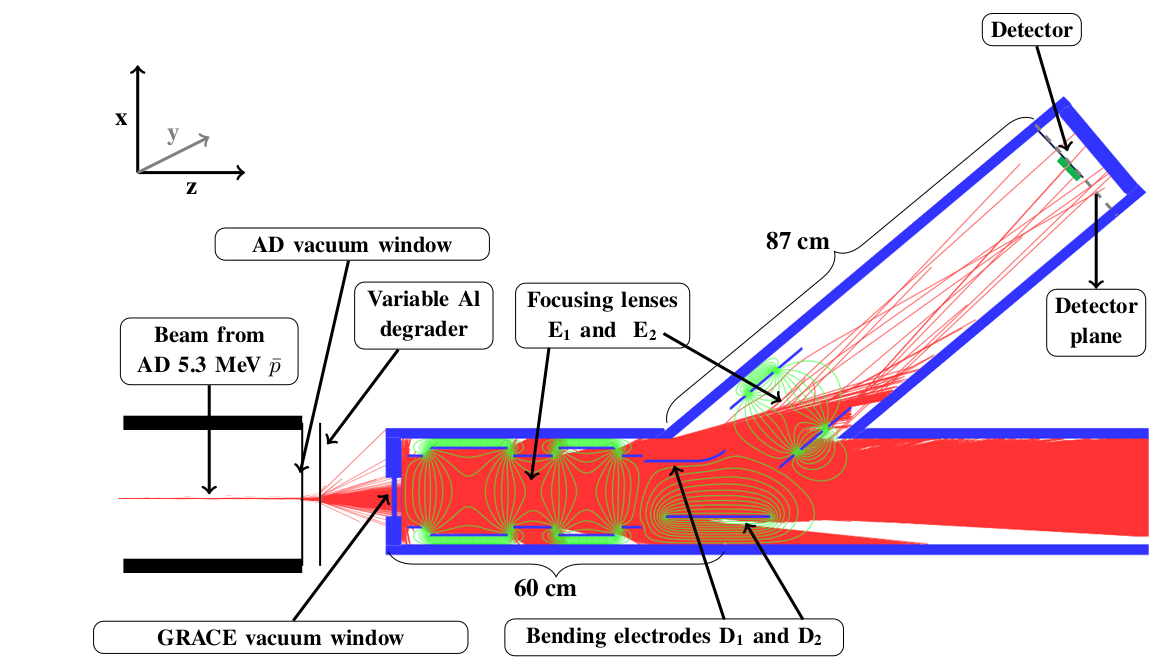
\includegraphics[width=\textwidth]{fig/Grace.png};
 \end{frame}



\begin{frame}{\centering The Timepix3 detector}
  \begin{columns}
    \begin{column}{0.5\textwidth}
      \begin{itemize}
      \item{670~$\mu$m thick}
      \item{55$\mu$m$\times$55$\mu$m pixels}
      \item{Self triggering pixels}
      \item{Measure both time of arrival and deposited energy}
      \item{Time resolution 1--2~ns}
      \end{itemize}
     \end{column}
    \begin{column}{0.5\textwidth}
      \begin{tikzpicture}
        \node at (0,0) {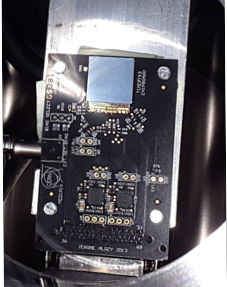
\includegraphics[width=\textwidth]{fig/MountedTimepix.png}};
        \visible<2>{\node at (0,0) [red,scale=8]{?};}
        \end{tikzpicture}
    \end{column}
  \end{columns}
 \end{frame}

\begin{frame}{\centering Antiproton data}
  %\begin{center}
  \vspace{-0.5cm}
  \begin{center}
    \only<1>{
      \resizebox{11.3cm}{8.3cm}{%
         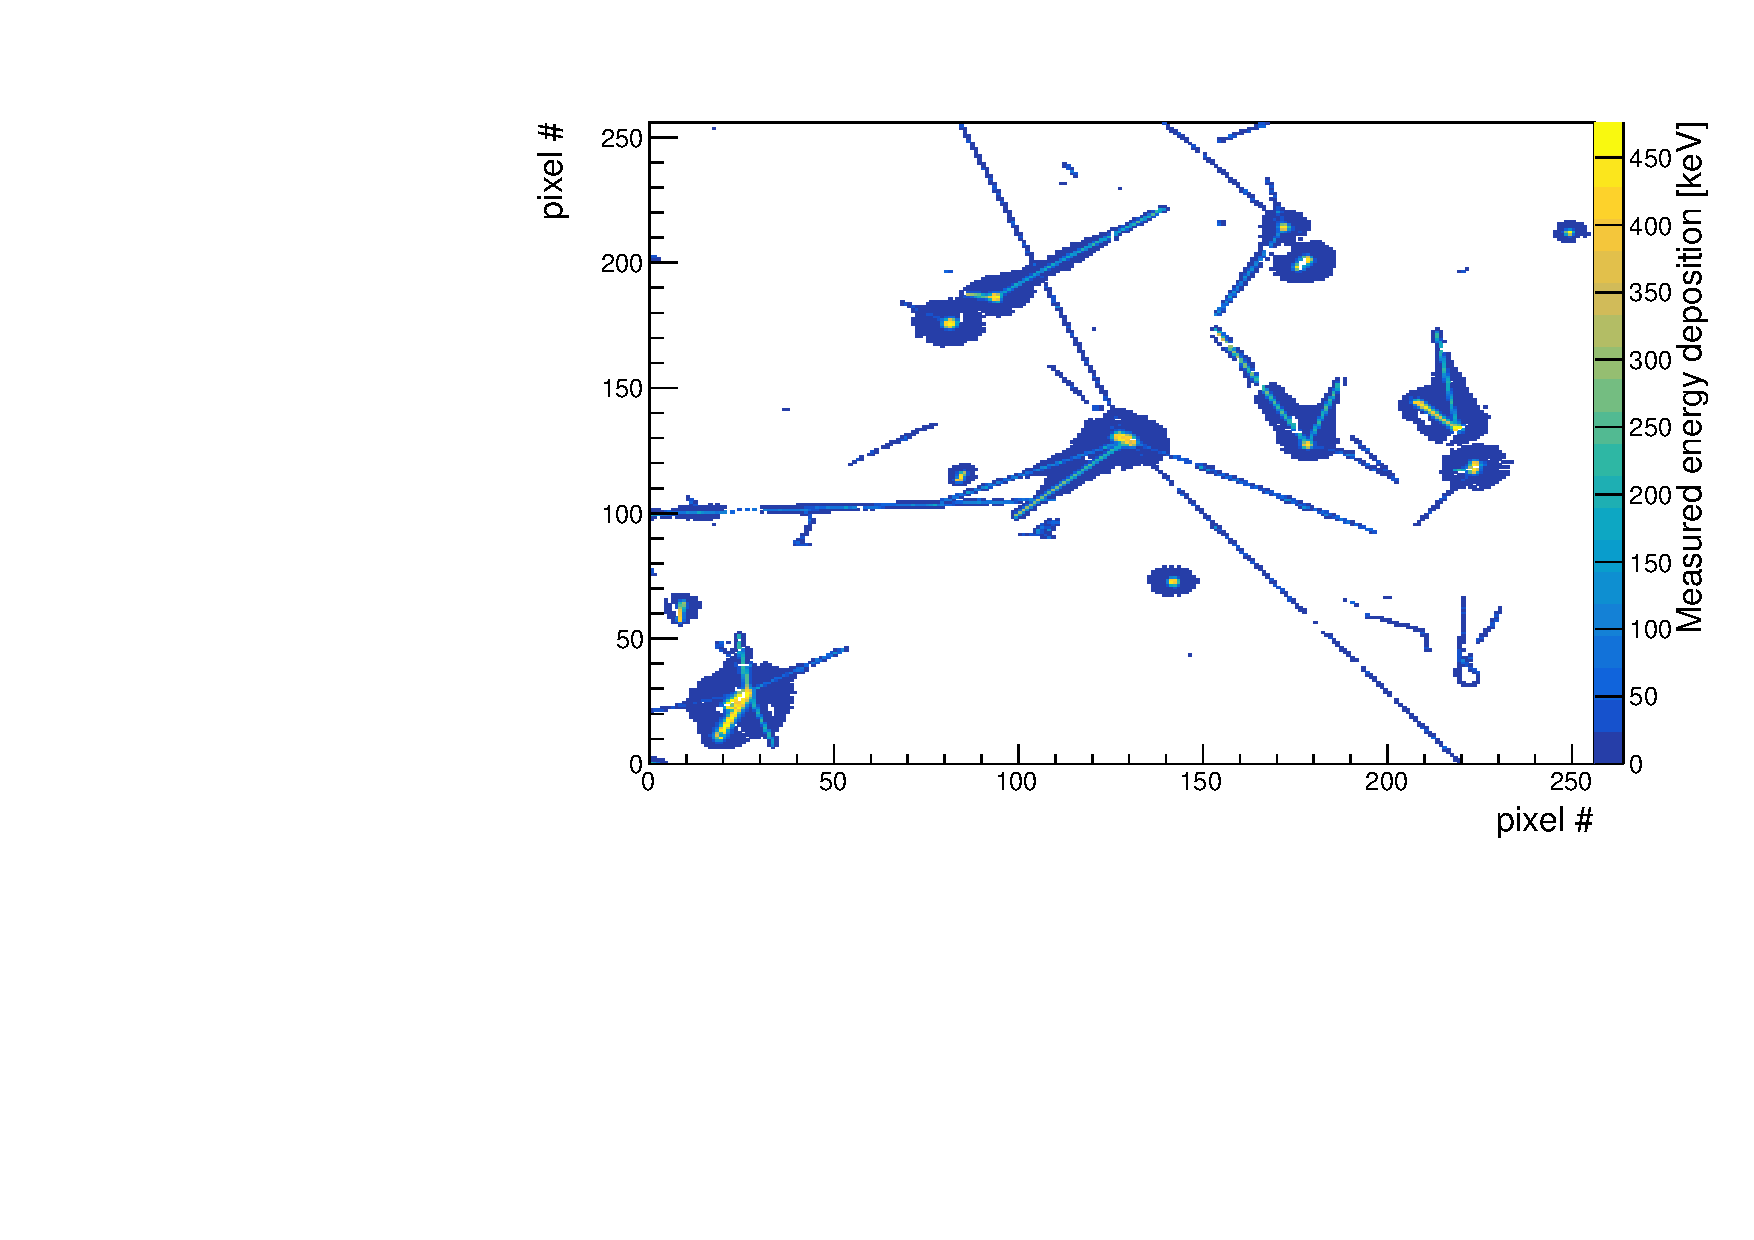
\includegraphics[width=5.0in]{fig/fullFrameUncleaned.pdf}
       }
       }
    \only<2>{
      \resizebox{11.3cm}{8.3cm}{%
    \begin{tikzpicture}
    \node[inner sep=0pt] (russell) at (0,0){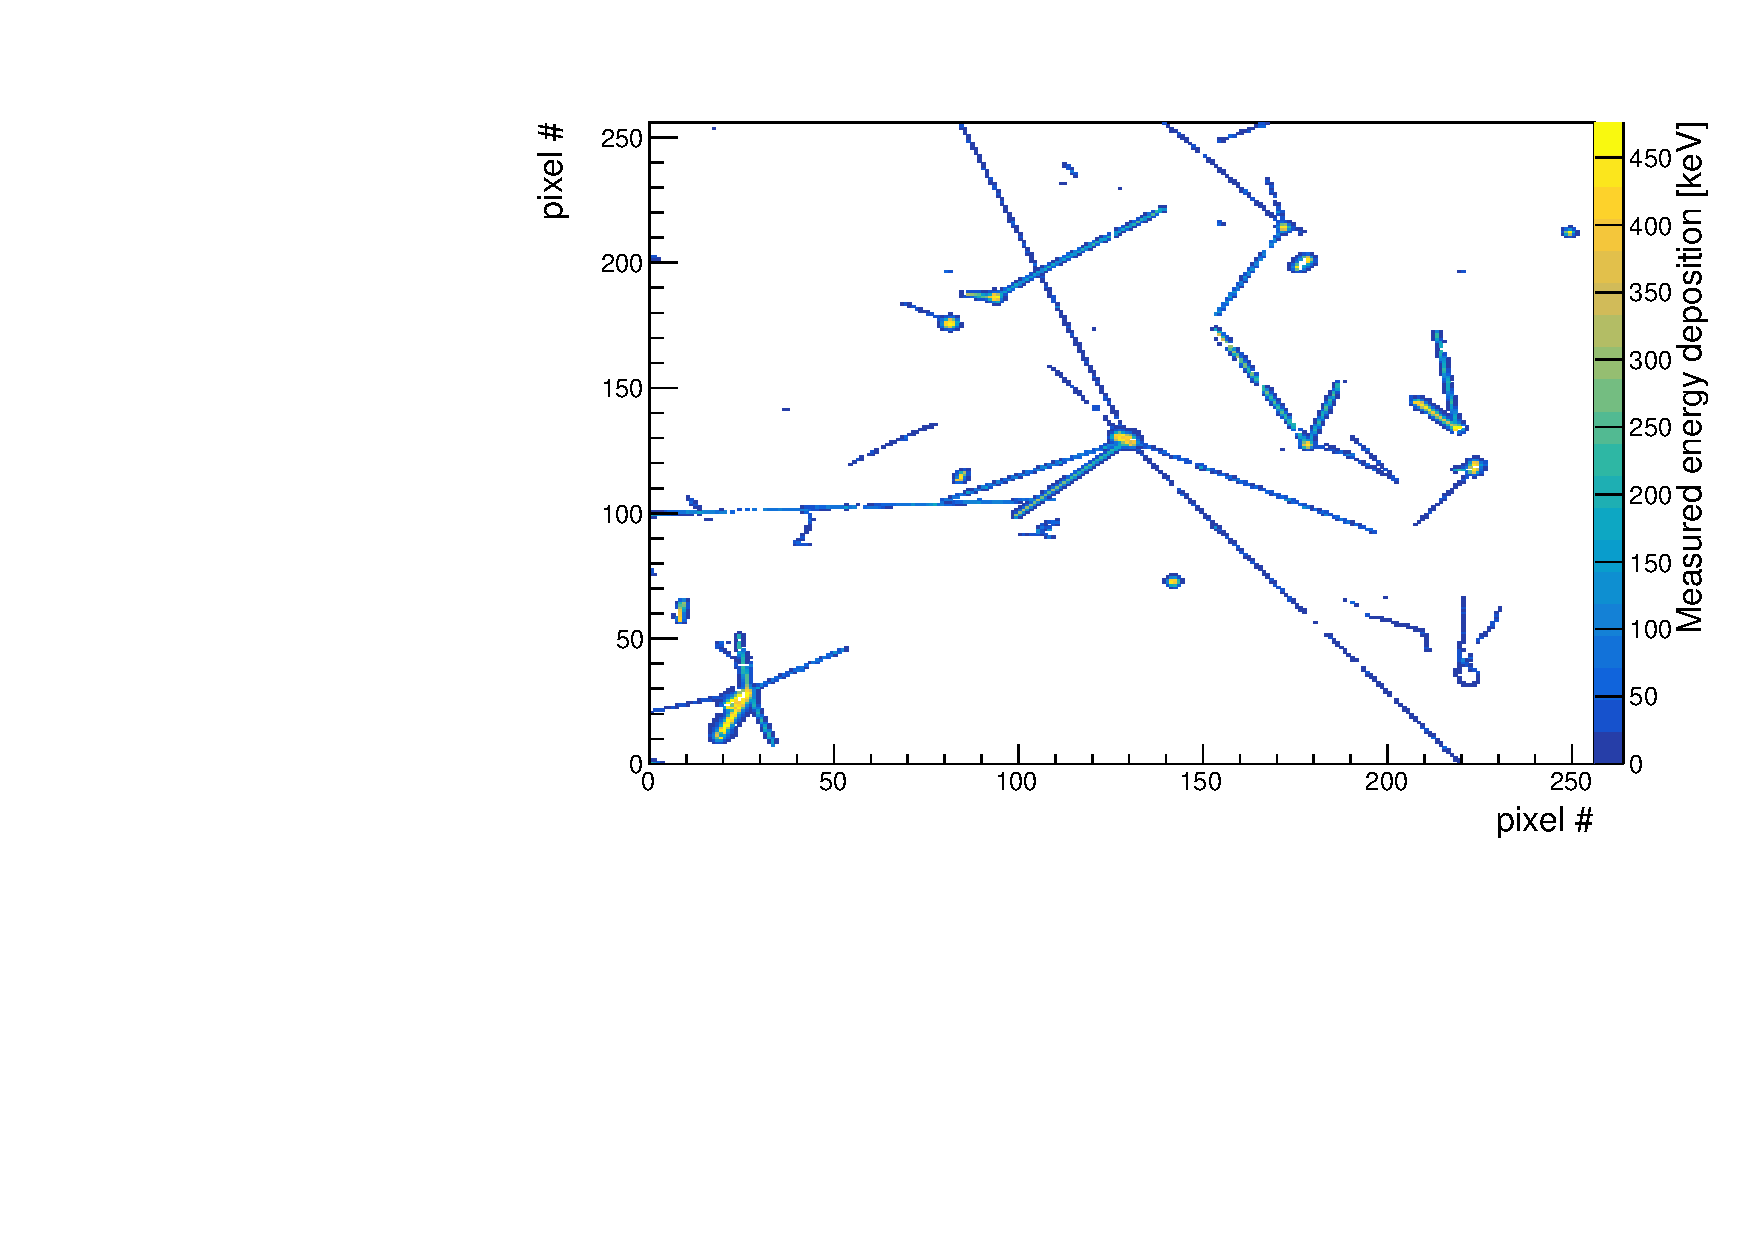
\includegraphics[width=5.0in]{fig/fullFrame.pdf}};
    %\draw [<-,black, thick] (-2.2,-1.6) to (-0.7,-2.0);
    %\draw [<-,black, thick] (0.03,-0.13) to (-0.5,-1.6);
    \node [rectangle,draw,text centered, rounded corners,text width=1.8cm,fill=white] at (-0.0,-2.7) (ann){\small Clear \\ annihilations };
    %\draw [<-,black, thick] (-1.2,0.9) to (-1.55,2.0);
    %\draw [<-,black, thick] (-0.9,1.1) to (-1.55,2.0);
    \node [draw,text width=2.0cm,text centered, rounded corners,fill=white] at (-3.45,2.9) (pani){\small Annihilation \\ candidates  };
    %\draw [<-,black, thick] (-1.7,0.1) to (-2.3,1.0);
    %\node [rectangle,text width=2.28cm,draw,text centered, rounded corners,fill=white,execute at begin node=\setlength{\baselineskip}{0.4em}] at (-4.5,0.6) (prob2) {\small Zero \\ \small prongs};
    %\node [rectangle,draw,text width=2.28cm,text centered, rounded corners,fill=white,execute at begin node=\setlength{\baselineskip}{0.4em}] at (3.4,2.95) (prob1) {\small Zero \\ \small prongs };
    \node [rectangle,text width=1.0cm,draw,text centered, rounded corners,fill=white] at (-4.5,0.6) (prob2) {\small Zero \\ \small prongs};
    \node [rectangle,draw,text width=1.0cm,text centered, rounded corners,fill=white] at (3.4,2.95) (prob1) {\small Zero \\ \small prongs };

    \path [line] (prob2)--(-2.5,0.05);
    \path [line] (prob1)--(2,2);
    \path  [line] (pani)--(-2.0,1.4);
    \path  [line] (pani)--(-1.6,1.7);
    \path  [line] (ann)--(-3.5,-2.55);
    \path  [line] (ann)--(0,-0.15);
    \end{tikzpicture}
    }
    }
    \end{center}
  %\end{center}
  %\hspace{10cm}
\end{frame}


\begin{frame}{\centering Analyse the data}
  \begin{columns}
    \begin{column}{0.45\textwidth}
      \begin{itemize}
      \item<1->{Clustering in time and space}
      \item<2->{Check for single tracks}
      \item<5->{Find and remove center}
      \item<7->{Hough transform to identify prongs}
      \item<8->{Remove prong}
      \item<9->{Find more prongs}
      \item<10>{Fit straight lines and find the intersection}
      \end{itemize}
    \end{column}
    \begin{column}{0.55\textwidth}
      %%       test
      \begin{tikzpicture}
        \only<1,2>{\node at (0,0){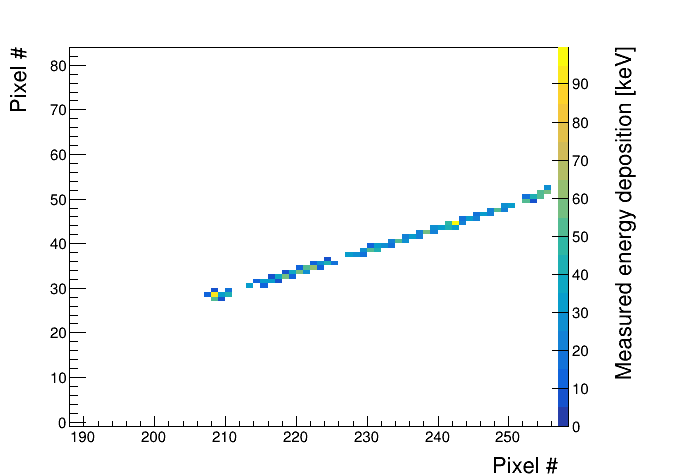
\includegraphics[width=2.55in]{fig/1060.png}};}
        \only<2>{\draw [thick,red](-2.8,-1)--(2.1,0.45);}
        \only<3,4>{\node at (0,0){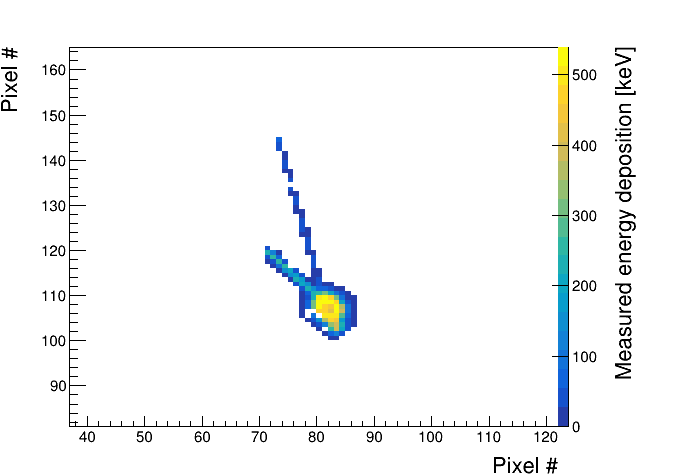
\includegraphics[width=2.55in]{fig/370.png}};}
        \only<4>{\draw [thick,red](-1.8,1.9)--(0.5,-1.9);}
        \only<5,6>{\node at (0,0){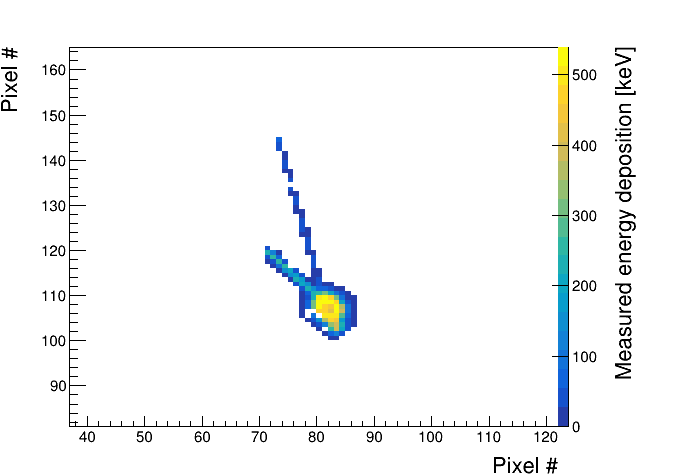
\includegraphics[width=2.55in]{fig/370.png}};}
        \only<5,6>{\draw[orange,thick] (-0.27,-0.78) circle (0.24);}
        \only<6>{\draw[black,thick,fill=black] (-0.22,-0.72) circle (0.03);}
        \only<7>{\node at (0,0){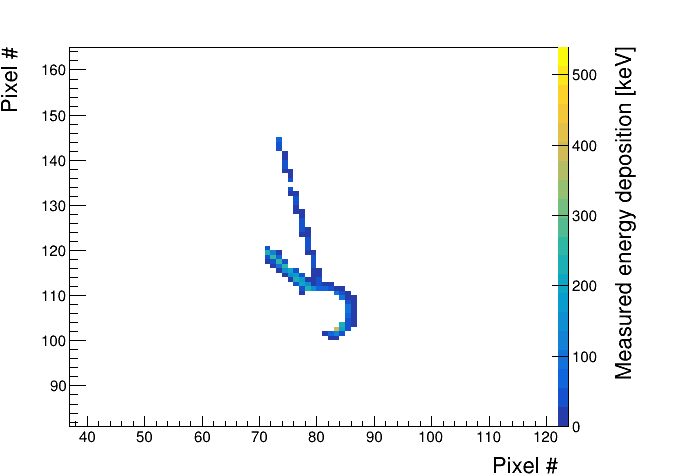
\includegraphics[width=2.55in]{fig/371.png}};}
        \only<7>{\draw[black,thick,fill=black] (-0.22,-0.72) circle (0.03);}
        \only<8>{\node at (0,0){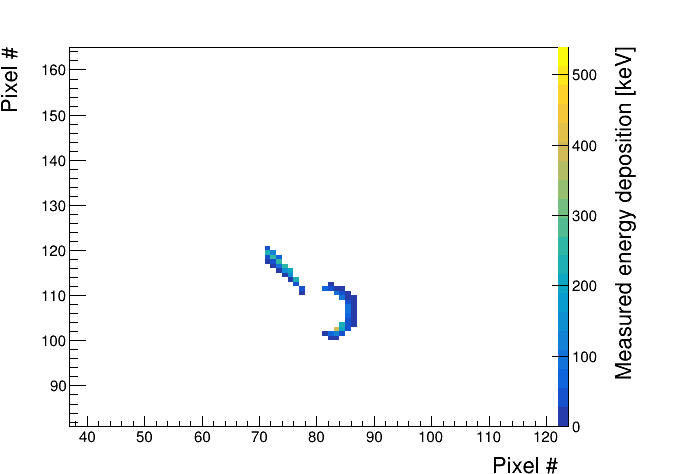
\includegraphics[width=2.55in]{fig/372.png}};}
%%    
        \only<9>{\node at (0,0){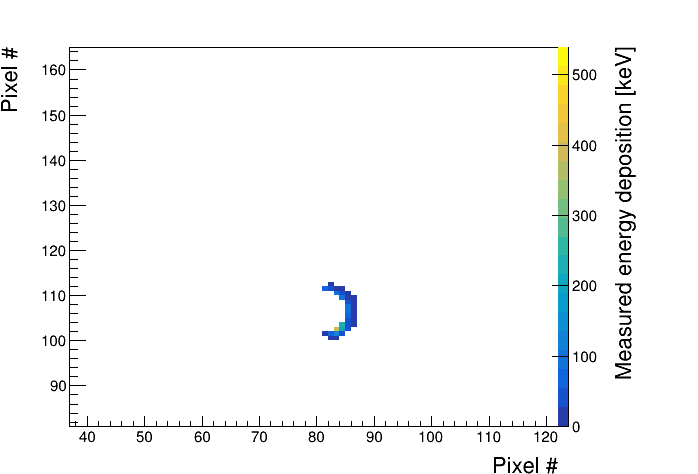
\includegraphics[width=2.55in]{fig/373.png}};}

        \only<10>{\node at (0,0){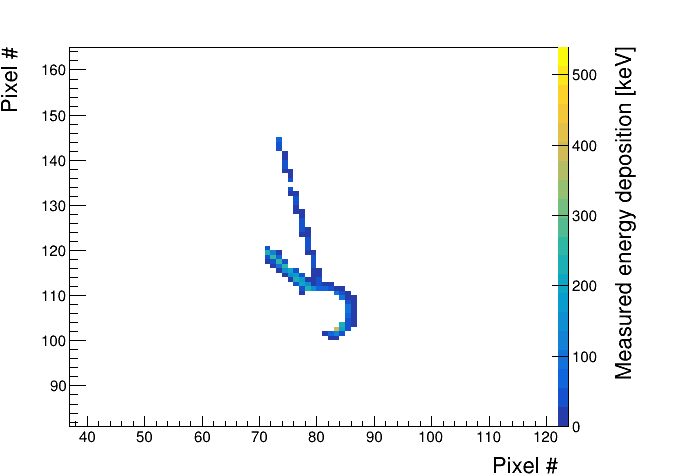
\includegraphics[width=2.55in]{fig/371.png}};}
        \only<10>{\draw [thick,green](-2.8,1.6)--(0.7,-1.45);}
        \only<10>{\draw [thick,green](-0.95,2)--(-0.0,-1.45);}
      \end{tikzpicture}
    \end{column}
  \end{columns}
\end{frame}


\begin{frame}{\centering Simulation of the detector}
  \begin{columns}
    \begin{column}{0.45\textwidth}
      \begin{itemize}
      \item<1->{Raw energy depositions in small voxels (FLUKA)}
      \item<2->{Parametrized model for charge sharing including the plasma effect}
      \item<3->{Volcano effect}
      \item<4->{Suppressed pixels in the experimental set-up}
      \item<4->{Re-clustering}
      \end{itemize}
    \end{column}
    \begin{column}{0.55\textwidth}
      \begin{tikzpicture}
      \only<1>{\node at (0,0){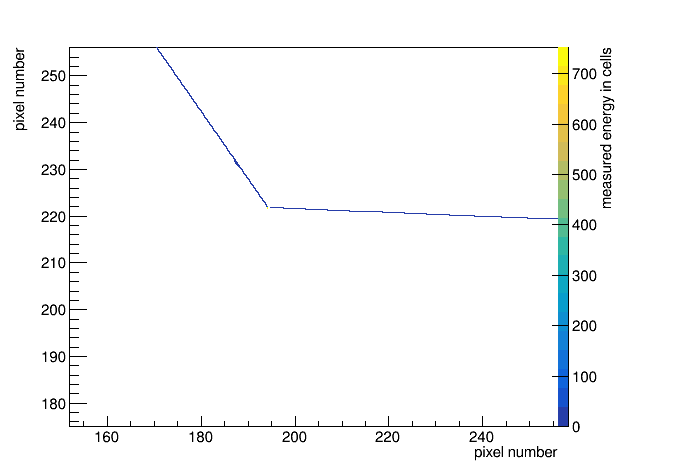
\includegraphics[width=2.55in]{fig/test/initial.png}}};
       \only<2>{\node at (0,0){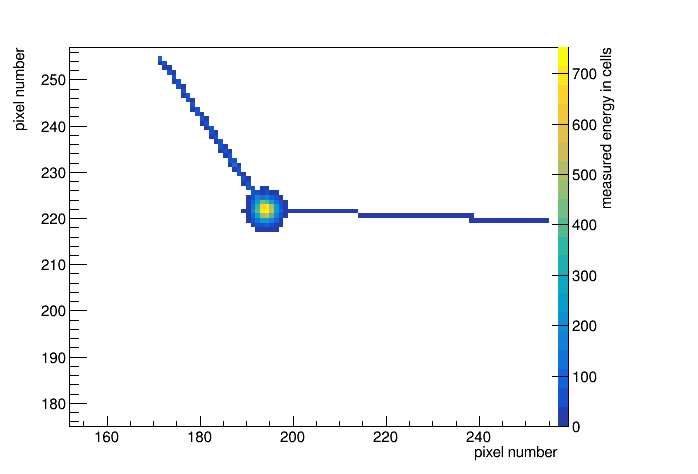
\includegraphics[width=2.55in]{fig/test/afterBlur.png}}};
      \only<3>{\node at (0,0){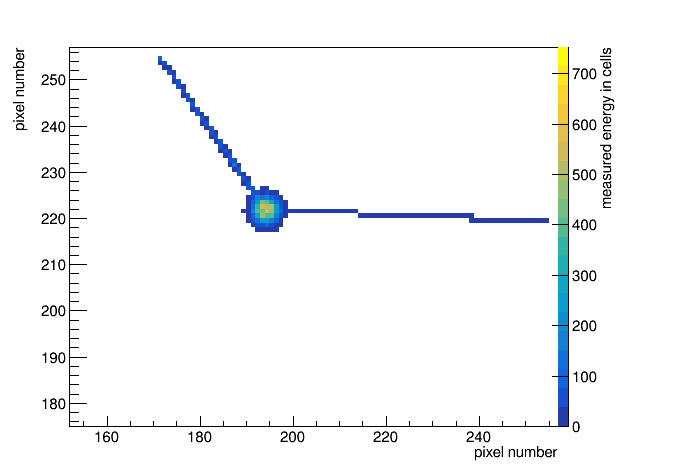
\includegraphics[width=2.55in]{fig/test/afterVolcano.png}}};
      \only<4>{\node at (0,0){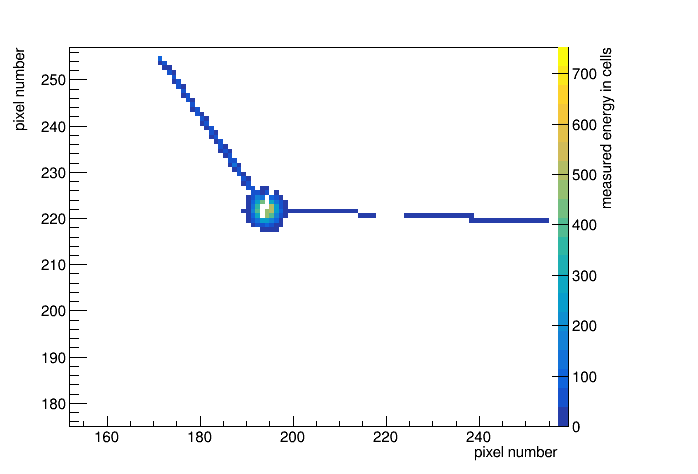
\includegraphics[width=2.55in]{fig/test/final.png}}};
      \end{tikzpicture}
    \end{column}
    \end{columns}
\end{frame}


\begin{frame}{\centering Verification of the simulation}
  \only<1>{\begin{block}{\centering Cluster energy}
    \centering
    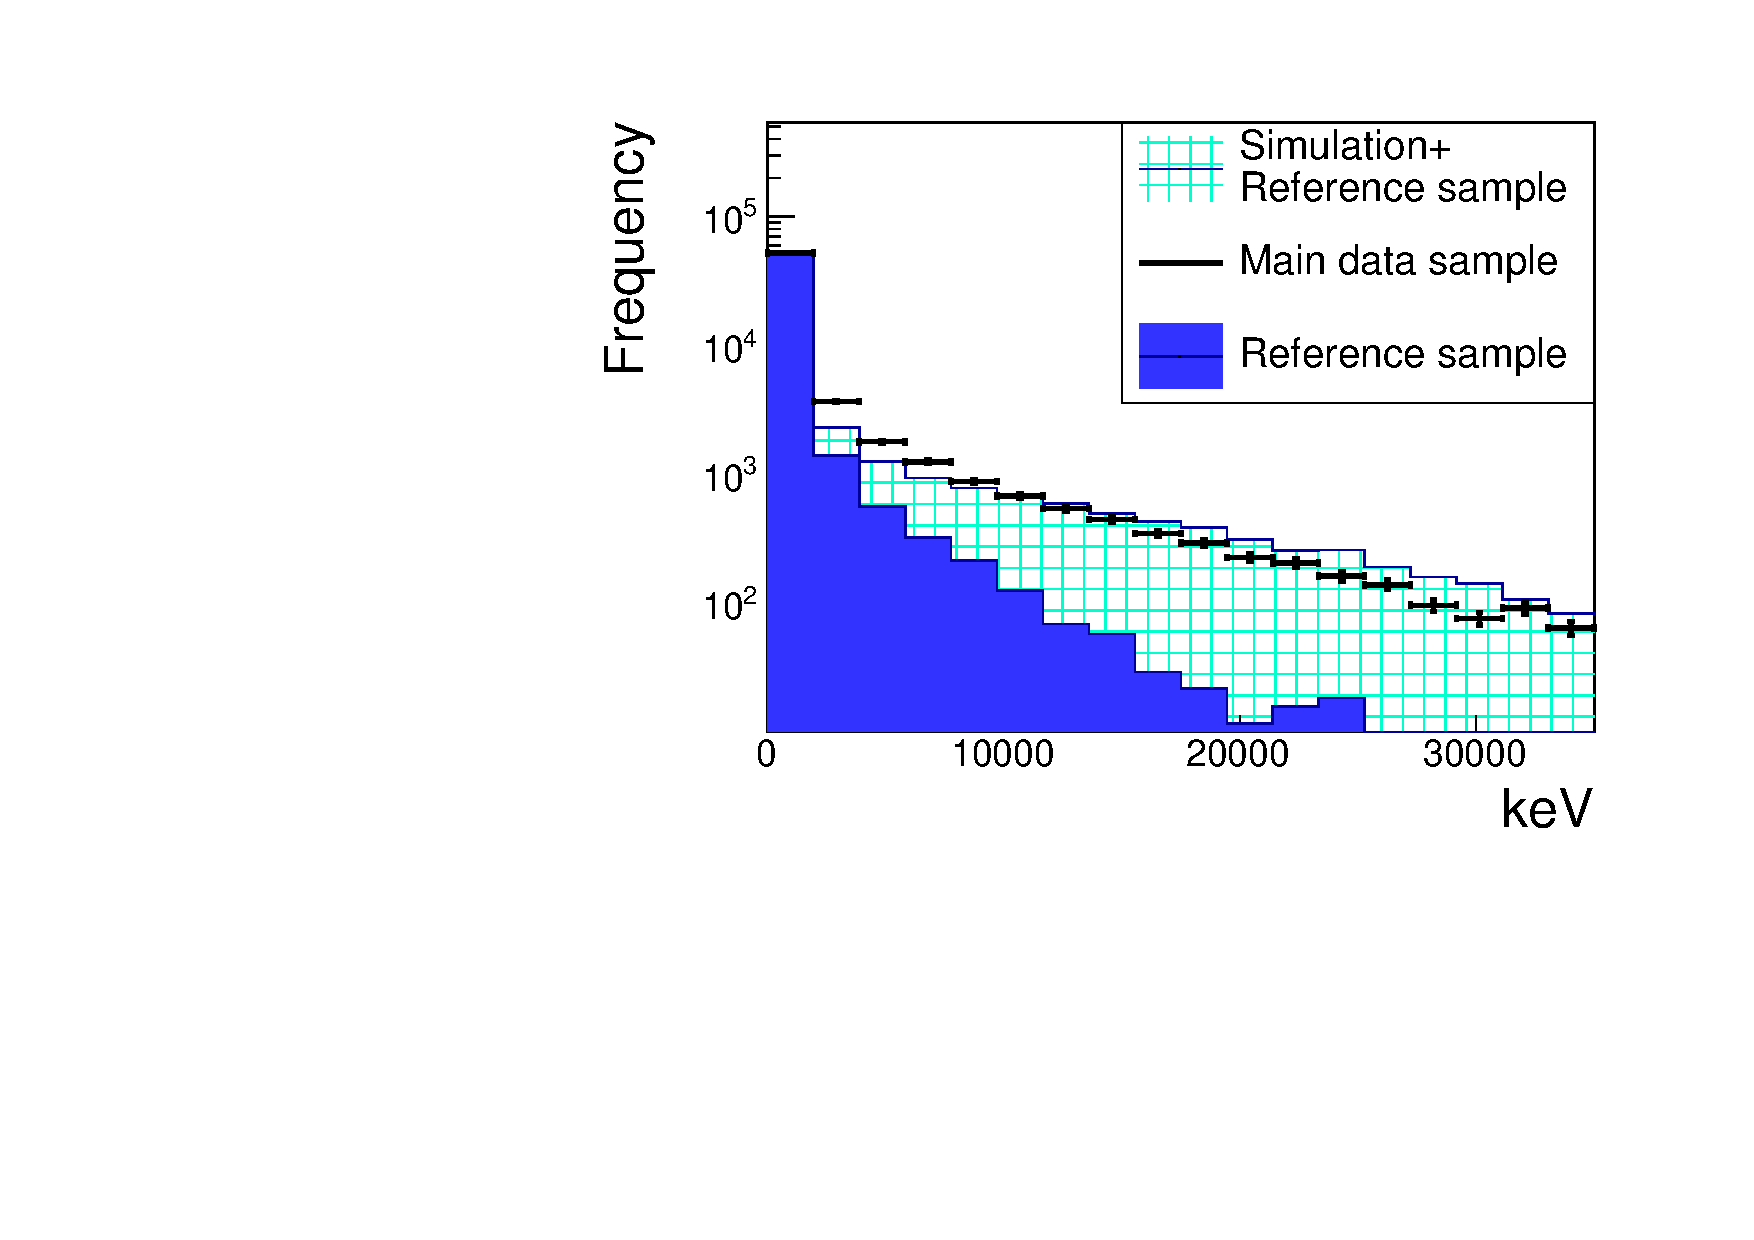
\includegraphics[width=3.55in]{fig/charge.pdf}
    \end{block}
  }
   \only<2>{\begin{block}{\centering Cluster energy in center}
    \centering
    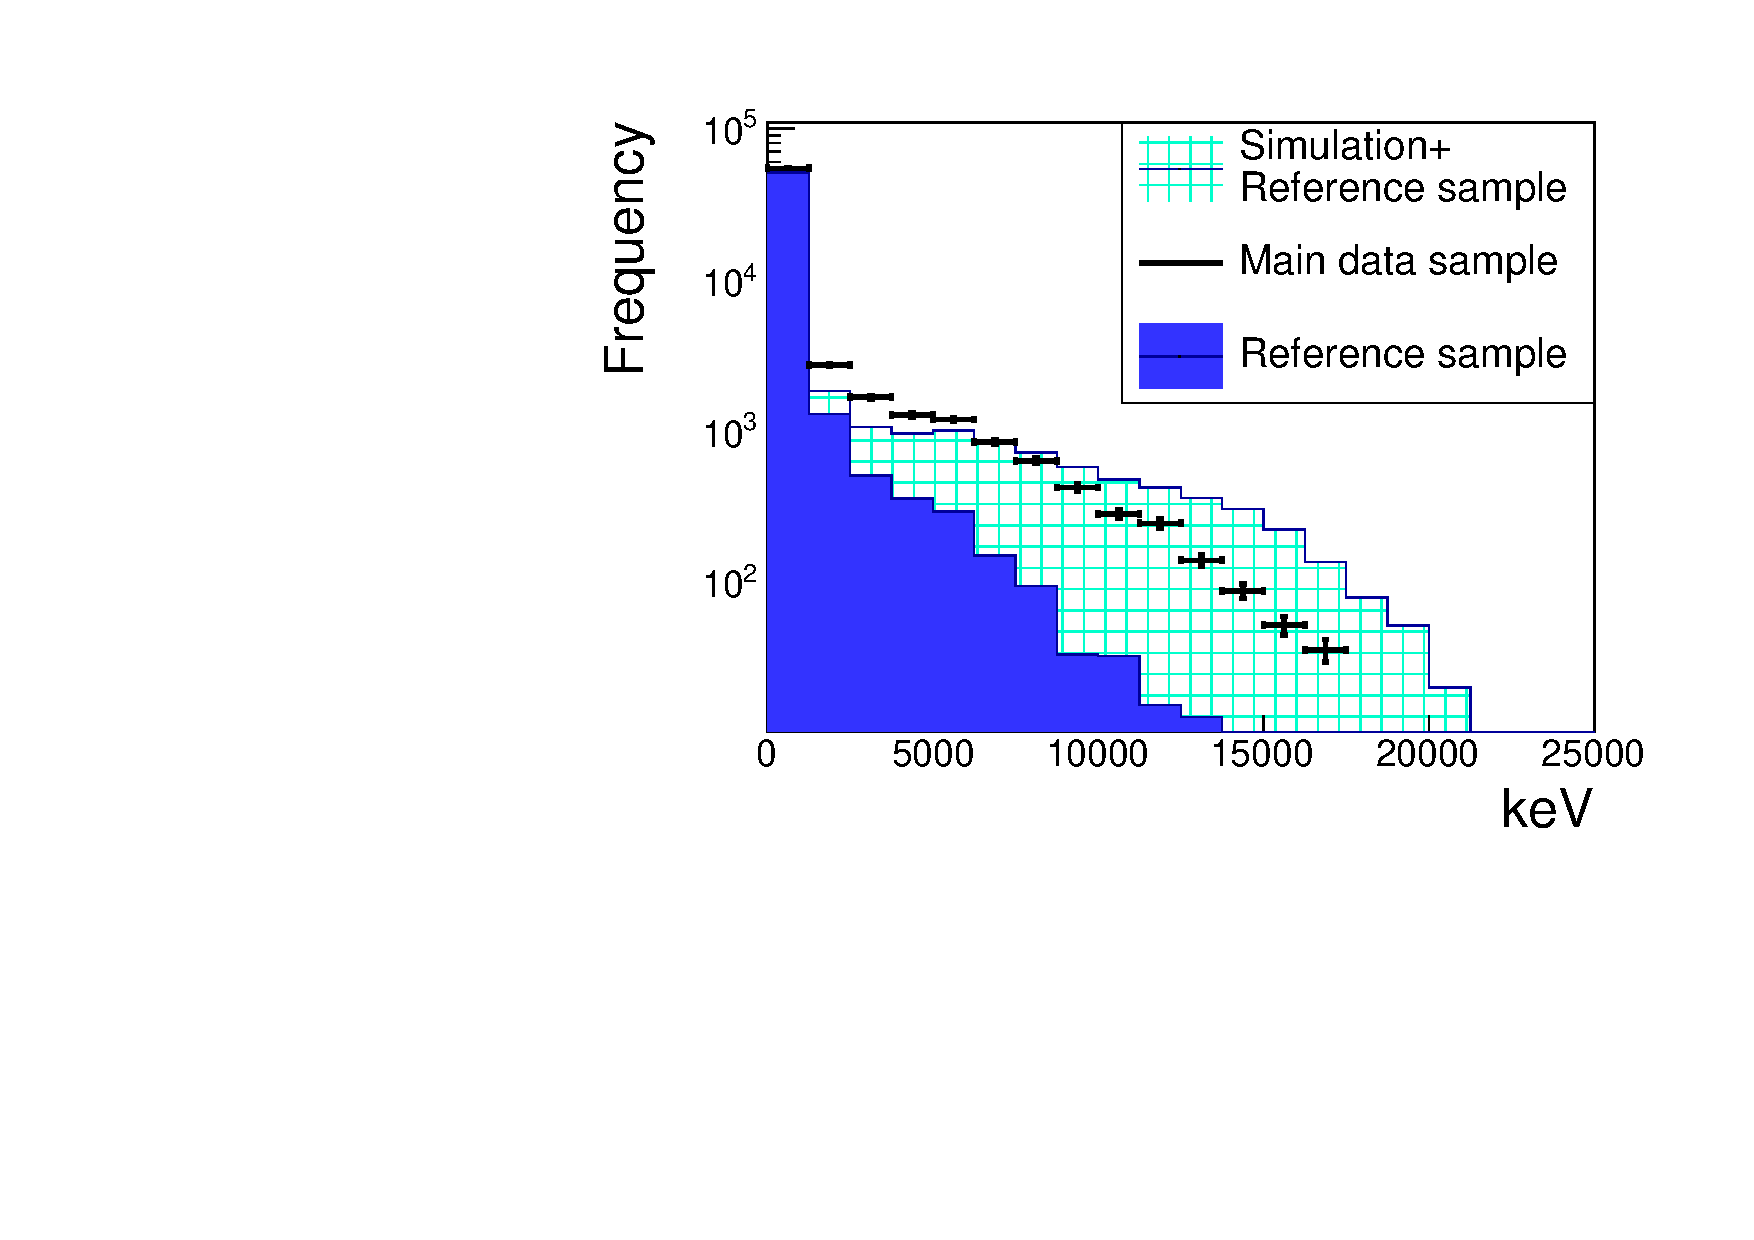
\includegraphics[width=3.55in]{fig/centerEnergy.pdf}
    \end{block}
   }
    \only<3>{\begin{block}{\centering Cluster size}
    \centering
    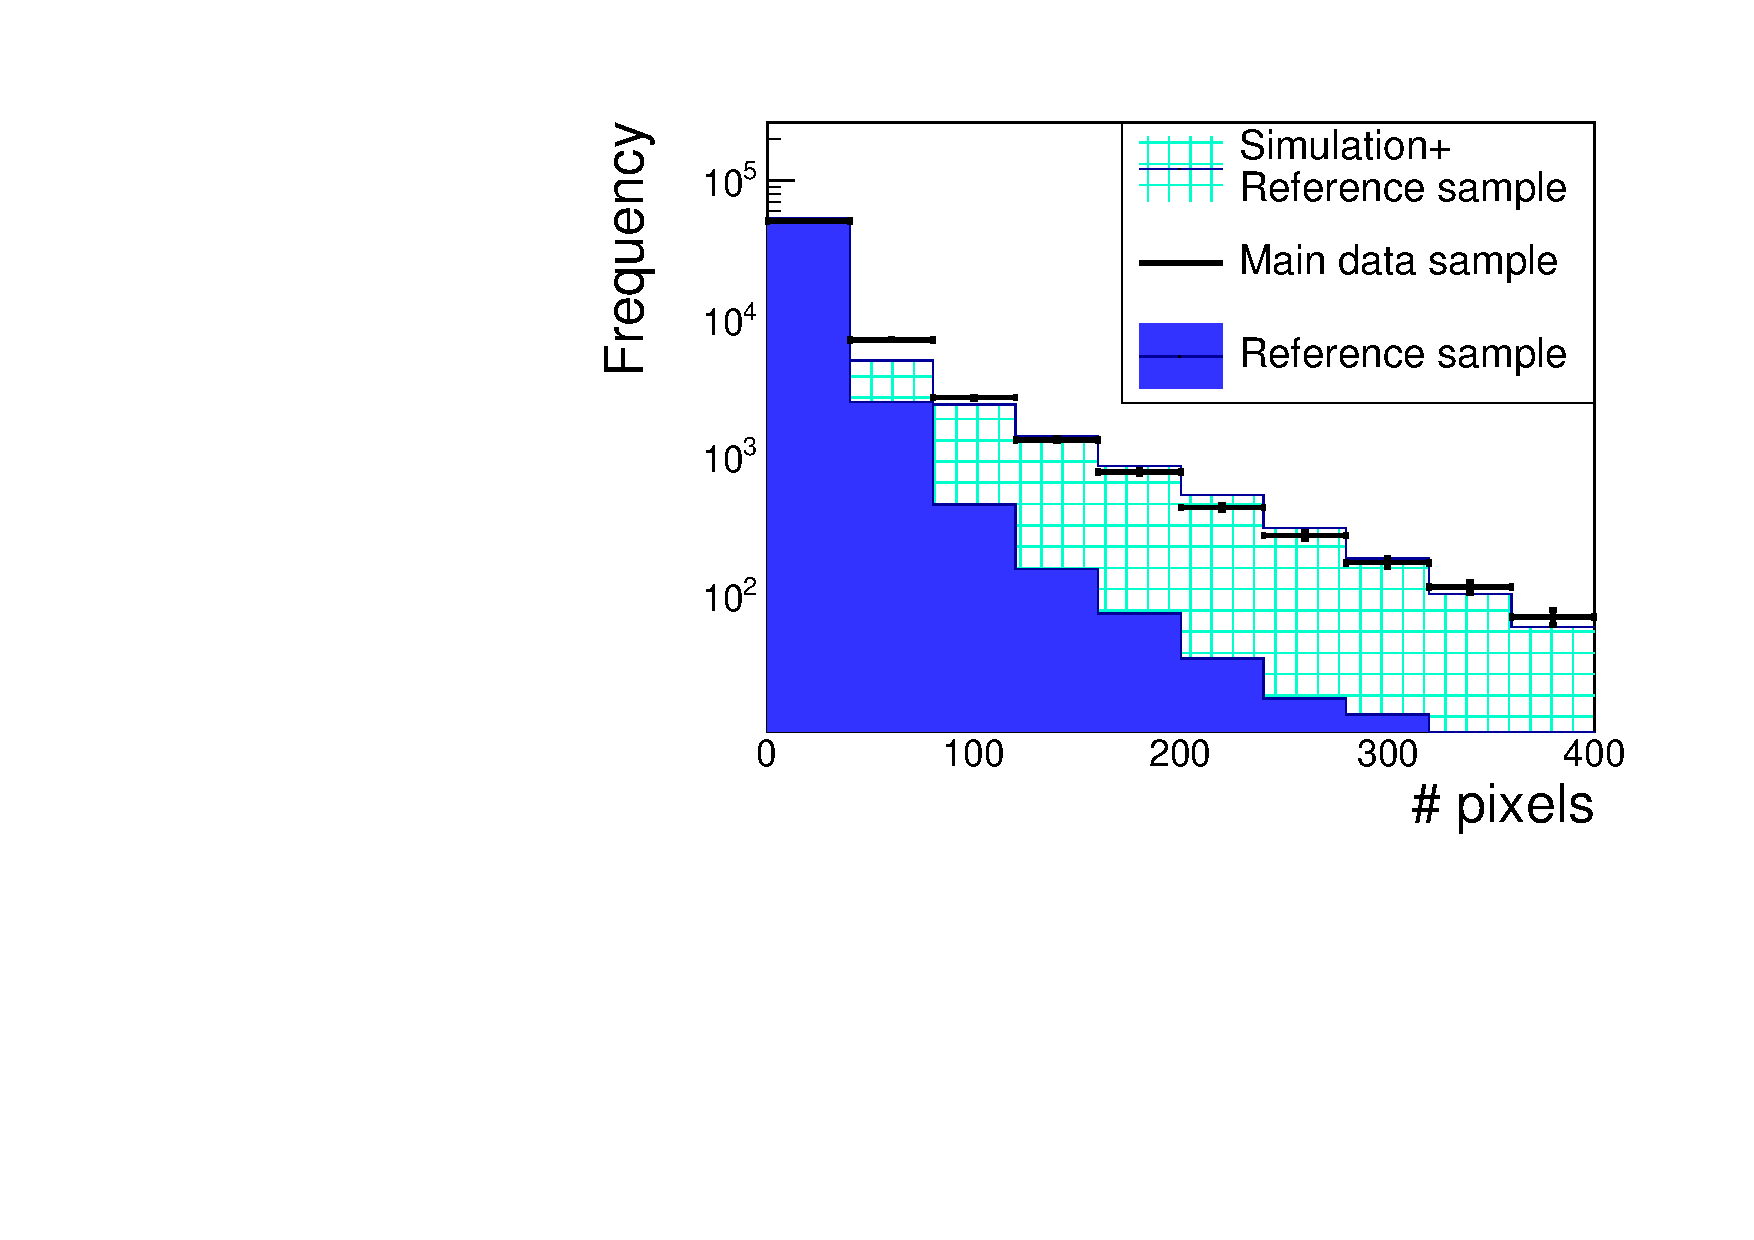
\includegraphics[width=3.55in]{fig/size.pdf}
    \end{block}
    }
     \only<4>{\begin{block}{\centering Number of prongs}
    \centering
    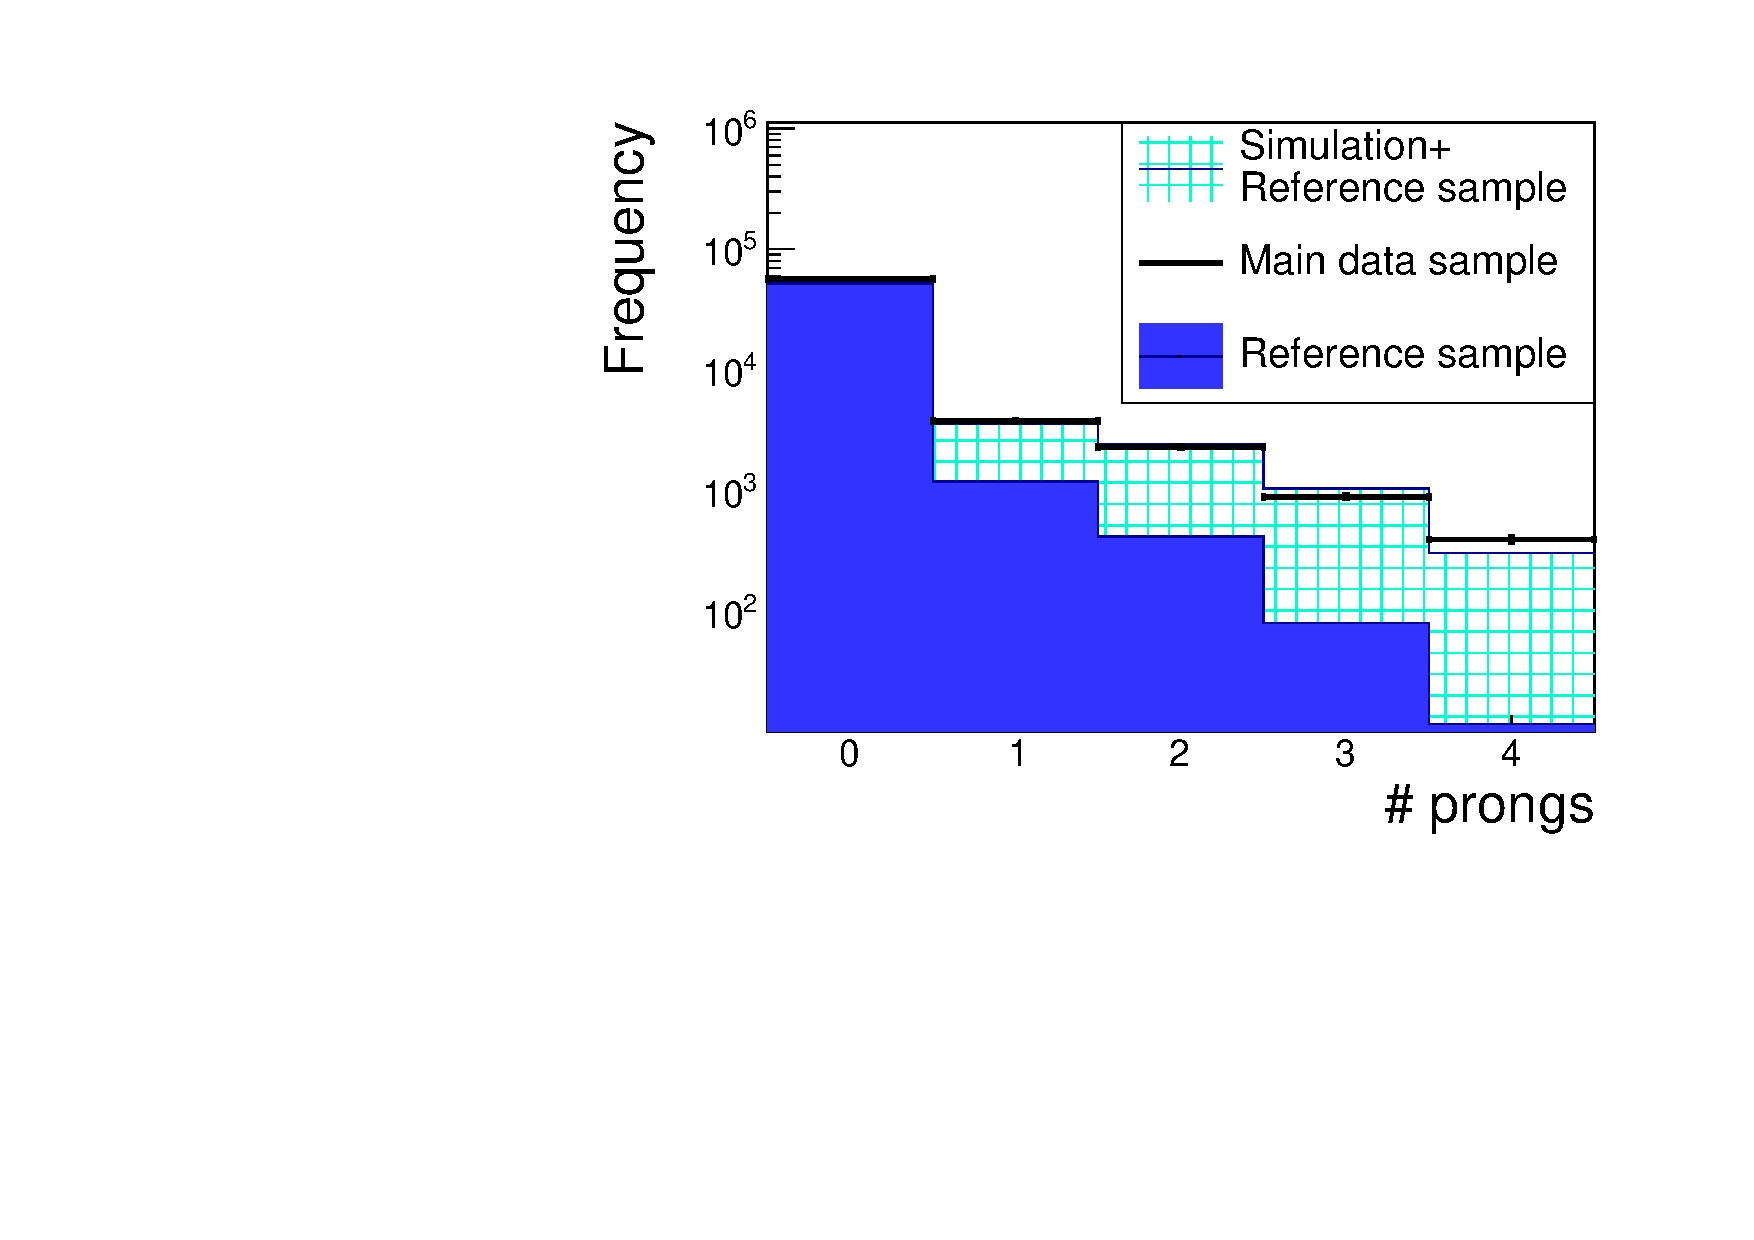
\includegraphics[width=3.55in]{fig/prongs.pdf}
    \end{block}
    }
\end{frame}



\begin{frame}{\centering Tagging efficiency}
 % \only<1>{\begin{block}{\centering}
  \centering
    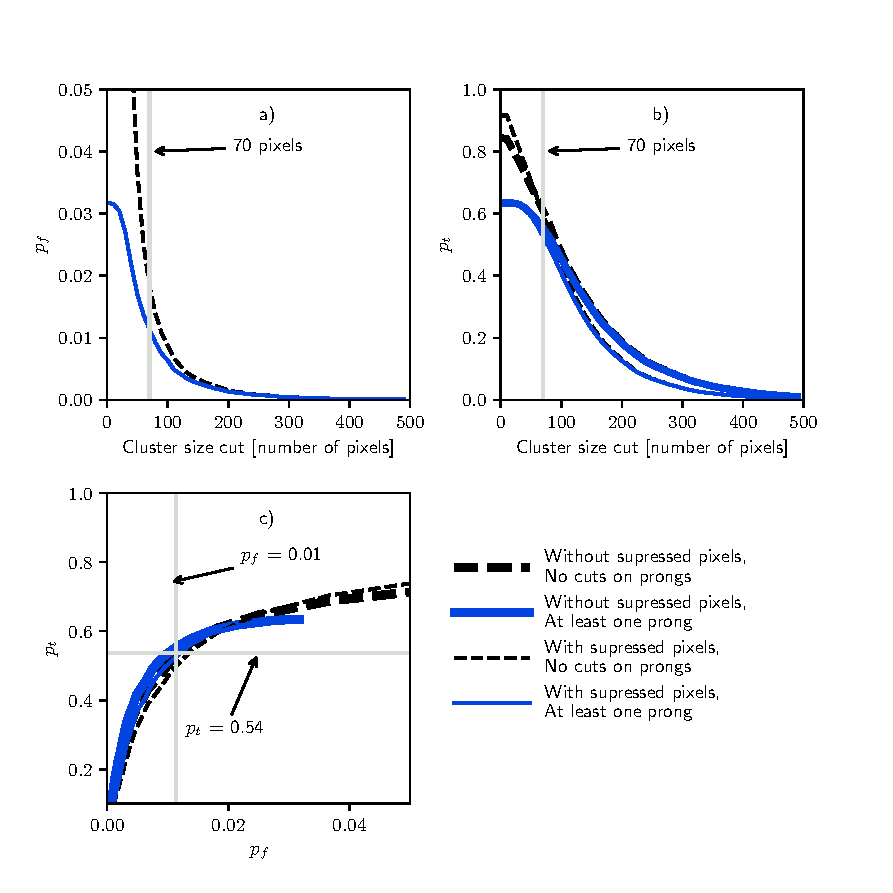
\includegraphics[width=3.17in]{fig/taggingEfficency}
%    \end{block}
%  }
\end{frame}
\begin{frame}{Position resolution}
  \begin{block}{\begin{itemize}
        \setlength{\itemindent}{2.5cm}
      \item{22 \% of the annihilations can be well reconstructed by the vertex fitting method}
      \item{Position resolution 22~$\mu$m}
      \end{itemize}
      }
      \centering
      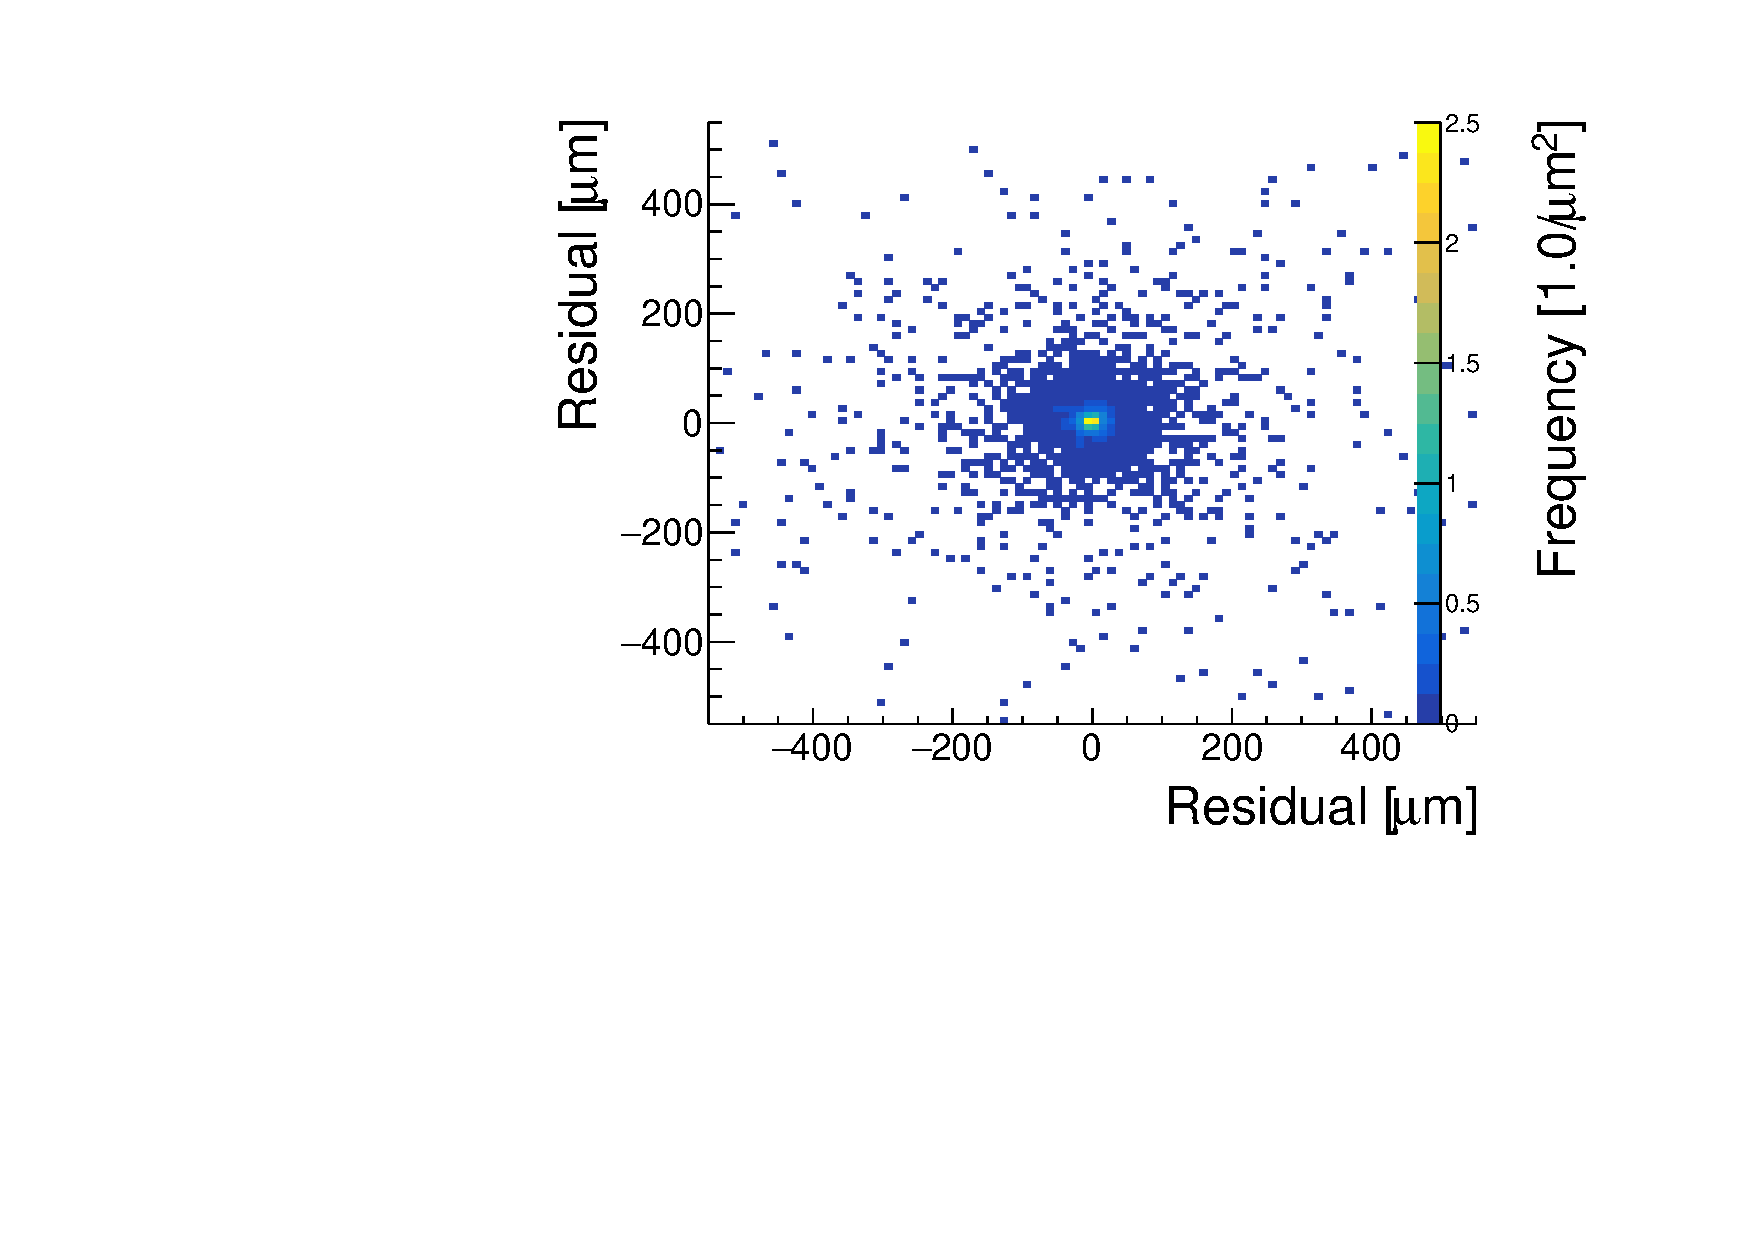
\includegraphics[width=3.25in]{fig/2dfit.pdf}
  \end{block}
\end{frame}

\begin{frame}{Conclusion}
  \begin{itemize}
  \item{We can clearly see the annihilation clusters}
  \item{Tagging efficiency of 50~$\pm$~10\%}
  \item{False positive rate $< 1$\%}
  \item{Position resolution of 22~$\mu$m}
  \end{itemize}
\end{frame}
  


\begin{frame}{For more information}  
  \begin{block}{Find all the details here}
    \vspace{0.1cm}
  \emph{Antiproton tagging and vertex fitting in a Timepix3 detector”
S. Aghion et al 2018 JINST 13 P06004}
  \href{http://iopscience.iop.org/article/10.1088/1748-0221/13/06/P06004}{link}.\\
  \vspace{0.3cm}
  \href{https://github.com/helgaholmestad/finalTimepix}{https://github.com/helgaholmestad/finalTimepix}.
  \end{block}
  \end{frame}
\begin{frame}{Thank you and goodbye!!}
  %\begin{block}{}
  % \centering{
    %Jerome Alozy~~Xavi Cudie\\
    %Michael Campbel~~Lukas Tlustos}
  \begin{block}{
      \begin{columns}
        \begin{column}{0.5\textwidth}
          \begin{itemize}
            \setlength{\itemindent}{1.4cm}
          \item{Jerome Alozy}
          \item{Michael Campbell}
          \end{itemize}
        \end{column}
        \begin{column}{0.5\textwidth}
          \begin{itemize}
          \item{Xavi Cudie}
          \item{Lukas Tlustos}
          \end{itemize}
        \end{column}
      \end{columns}
    }
    \centering
    \vspace{0.5cm}
       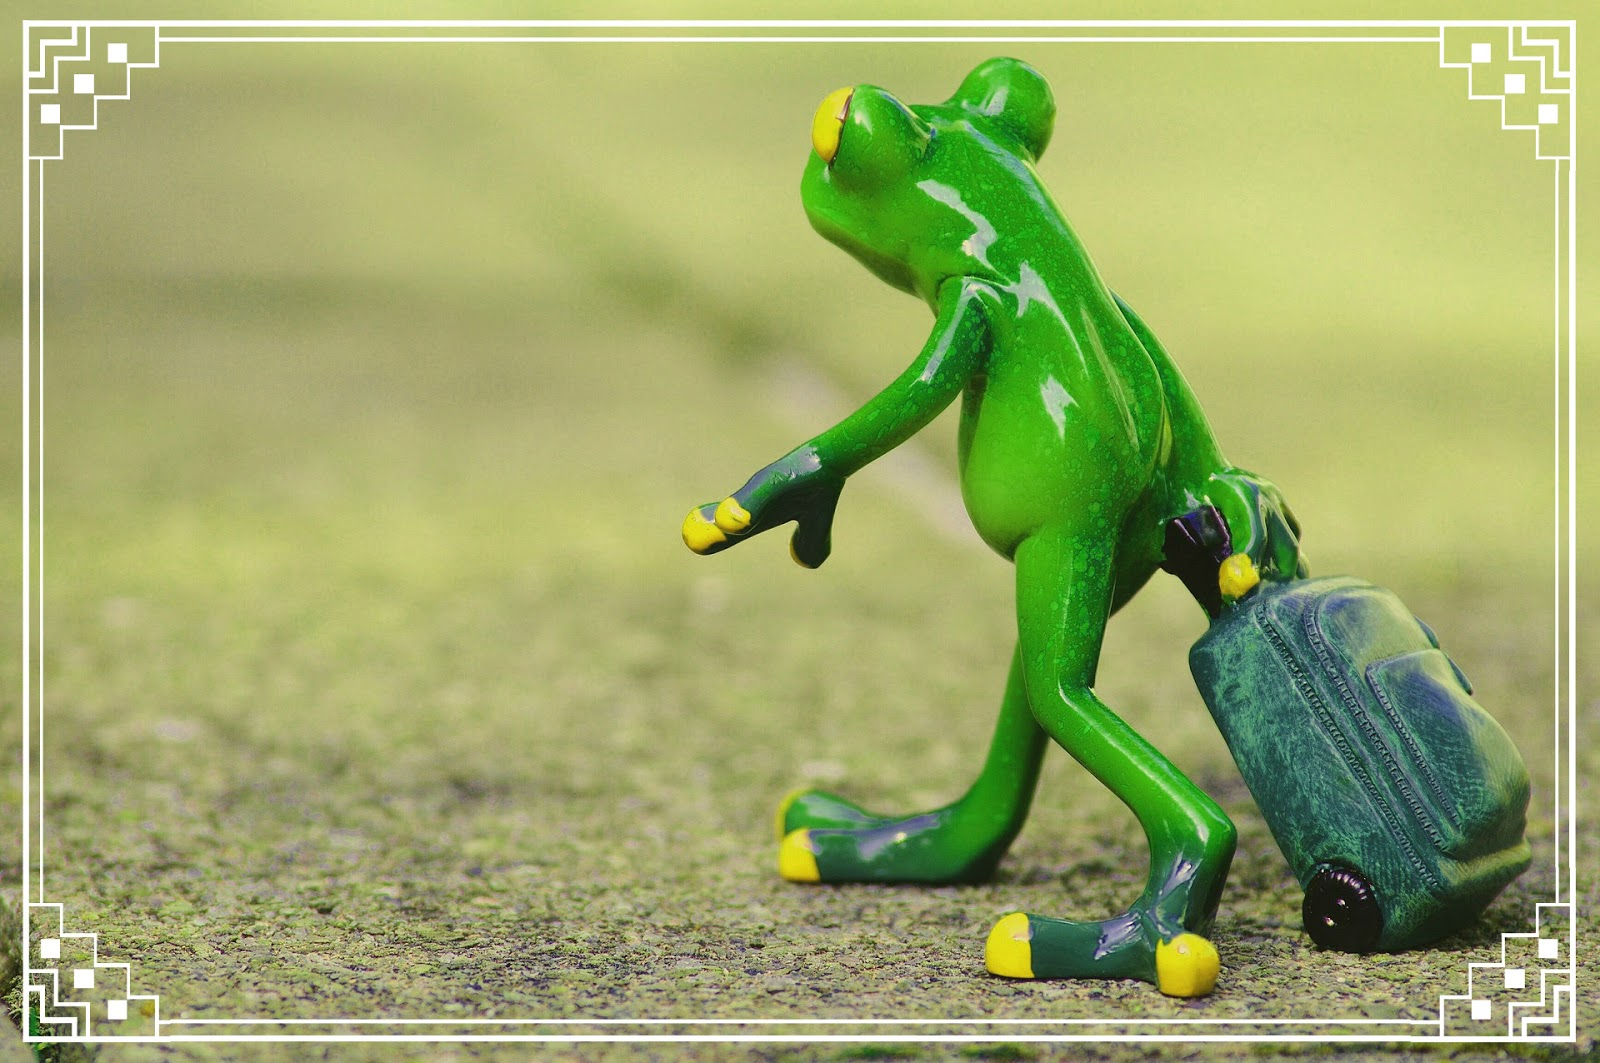
\includegraphics[width=3.00in]{fig/OnVacation.jpg}
  \end{block}
 %%  \begin{frame}{Thank you and goodbye!!}
 %%  %\begin{block}{}
 %%  % \centering{
 %%    %Jerome Alozy~~Xavi Cudie\\
 %%    %Michael Campbel~~Lukas Tlustos}
 %%  \begin{block}{\begin{itemize}
 %%        \setlength{\itemindent}{2.5cm}
 %%      \item{Jerome Alozy~~~~~~~~Xavi Cudie}
 %%      \item{Michael Campbell~~Lukas Tlustos}
 %%     \end{itemize}
 %%     }
 %%    \centering
 %%    \vspace{0.5cm}
 %%       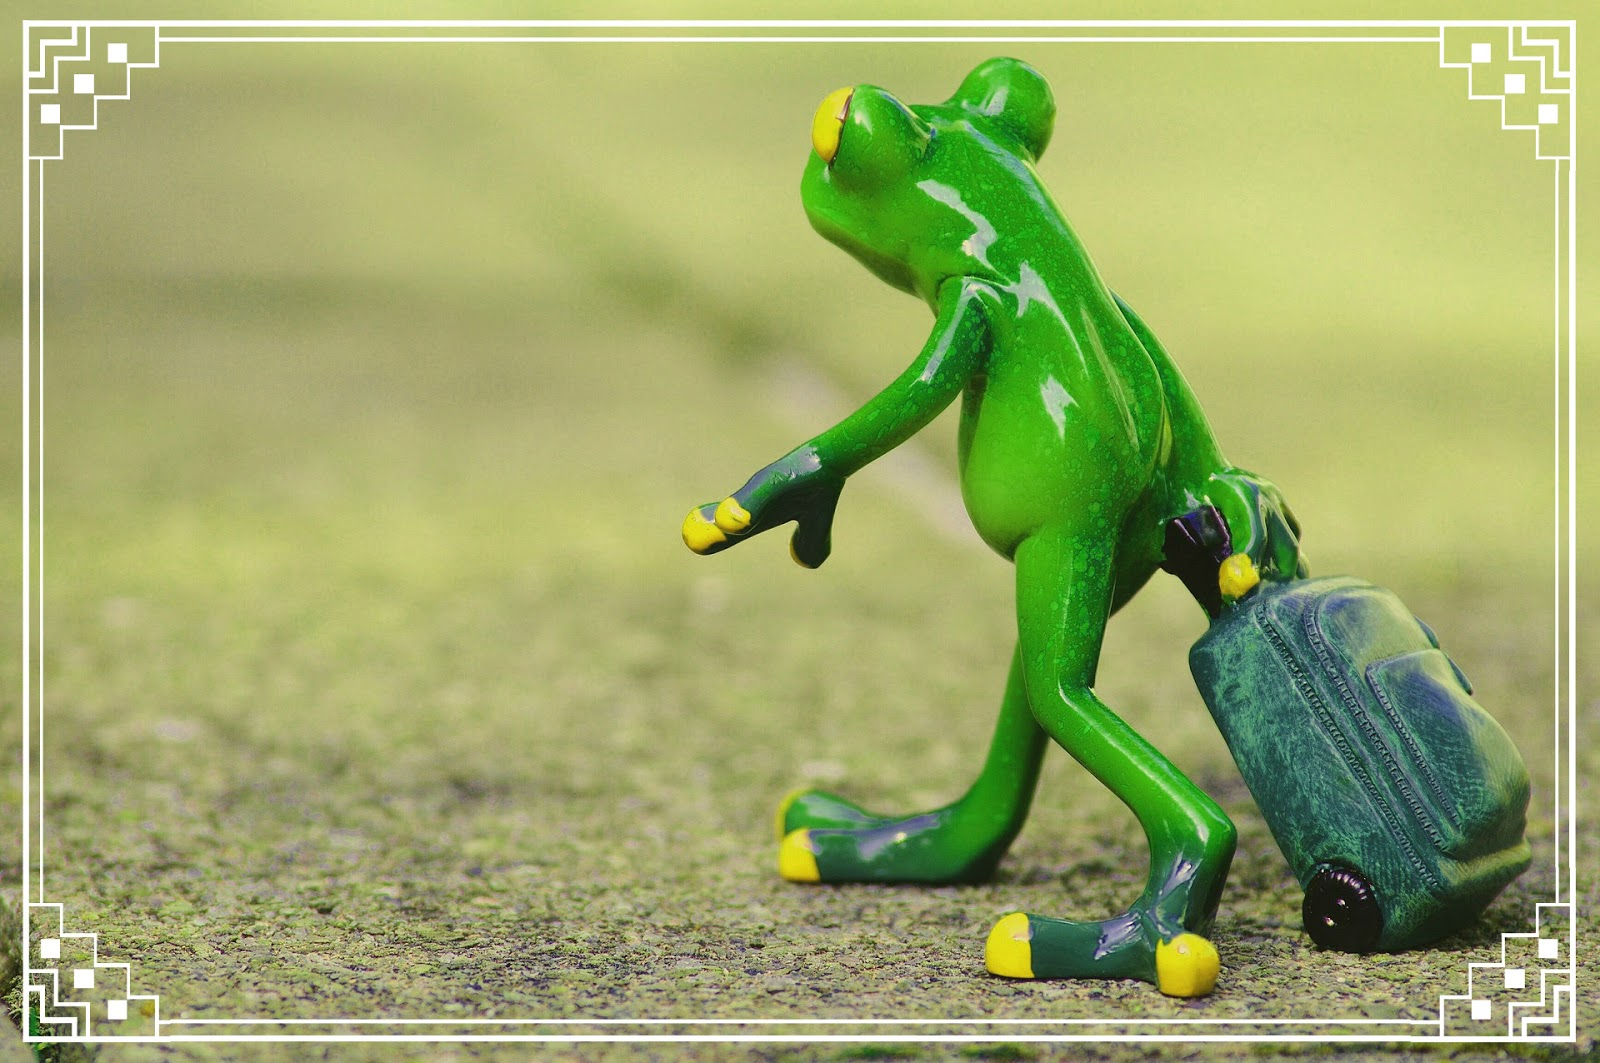
\includegraphics[width=3.00in]{fig/OnVacation.jpg}
 %% \end{block}
\end{frame}
\end{document}
